% !TEX encoding = UTF-8 Unicode

\documentclass[a4paper]{article}

\usepackage{color}
\usepackage{url}
\usepackage[T2A]{fontenc} % enable Cyrillic fonts
\usepackage[utf8]{inputenc} % make weird characters work
\usepackage{graphicx}
\usepackage{subfig}

\usepackage[english,serbian]{babel}
%\usepackage[english,serbianc]{babel} %ukljuciti babel sa ovim opcijama, umesto gornjim, ukoliko se koristi cirilica

\usepackage[unicode]{hyperref}
\hypersetup{colorlinks,citecolor=green,filecolor=green,linkcolor=blue,urlcolor=blue}

%\newtheorem{primer}{Пример}[section] %ćirilični primer
\newtheorem{primer}{Primer}[section]

\begin{document}

\title{Eliminacija pozadine u video zapisima\\ \small{Seminarski rad u okviru kursa\\Naučno izračunavanje\\ Matematički fakultet}}

\author{\href{mailto:mi14097@matf.bg.ac.rs}{Vesna Katanić}, \href{mailto:mi14022@matf.bg.ac.rs}{Anja Ivanišević}}
\date{14.~septembar 2019.}
\maketitle

\tableofcontents

\newpage

\section{Uvod}
\label{sec:uvod}

Algoritmi za eliminaciju pozadine u video zapisima su algoritmi koji imaju za cilj detekciju kretanja i odvajanje pozadine od objekata koji se kreću. CIlj ovog rada je upoznavanje različitim algoritmima za detekciju kretanja i njihovo poređenje.

\section{Primenjeni algoritmi}
\label{sec:algoritmi}

U ovom radu smo poredili tri različita algoritma za eliminaciju pozadine u video zapisima. Ti algoritmi su: \emph{Basic Motion Detection (BMD)}, \emph{Gaussian Mixture Model (GMM)} i \emph{K Nearest Neighbours (KNN)}. Ideja svakog od ovih algoritama je da transformišu ulazni video u novi video u kojem će pozadina biti ofarbana u crno a objekti koji se kreću u belo, kako bi se oni izdvojili. U nastavku rada će ovi algoritmi biti predstavljeni.

\subsection{Basic Motion Detection}

\emph{Basic Motion Detection} je najjednostavniji algoritam od predstavljenih algoritama. U ovom algoritmu se polazi od pretpostavke da se video $I$ sastoji od statičke pozadine $B$ ispred koje se nalaze objekti koji se kreću. Kako bismo detektovali objekte računa se rastojanje trenutnog modela pozadine i posmatranog frejma. Na osnovu ovog rastojanja pravi se rezultujuća crno-bela slika. 

Model pozadine se ažurira na osnovu prethodnog stanja i trenutno posmatranog frejma po sledećoj formuli: 
$B_{s,t+1} = (1 - \alpha) * B_{s,t} + \alpha * I_{s,t}$
gde je $s$ posmatrani piksel, $t$ posmatrani frejm i $\alpha$ parametar za koju je uzeta vrednost $0.001$. Za početnu vrednost modela pozadine $B$ je uzet prvi frejm, dok je rastojanje između frejma i modela računato na osnovu Euklidskog rastojanja.

\subsection{Gaussian Mixture Model}

Ideja algoritma \emph{Gaussian Mixture Model} je da imamo $K$ klastera. Za svaki klaster računamo matematičko očekivanje i stanardnu devijaciju Gausove raspodele i njihovim kombinovanjem modelujemo svaki piksel. Broj $K$ se određuje za svaki piksel posebno. Implementacija ovog algoritma postoji u OpenCV biblioteci i nju smo koristili za potrebe ovog rada.

\subsection{K Nearest Neighbours}

Ideja ovog algoritma je da se konstantno ažuriraju parametri Gaussian Mixture Modela i bira odgovarajući broj komponenti za svaki piksel. Koristi se metoda K najbližih suseda. Implementacija ovog algoritma postoji u OpenCV biblioteci i nju smo koristili za potrebe ovog rada.


\section{Evaluacija algoritma}
\label{sec:efikasnost}

Na narednim slikama su redom prikazani ulazna slika i rezultati algoritama \emph{BMD}, \emph{GMM} i \emph{KNN}.


\begin{figure}
    \centering
    \subfloat[Original]{{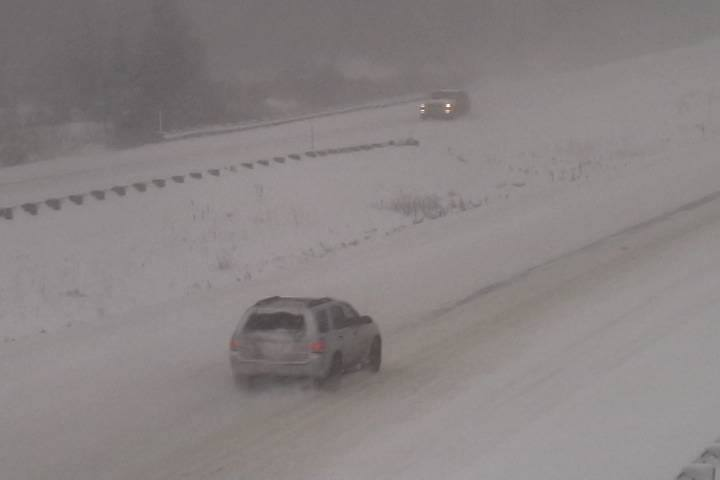
\includegraphics[width=5cm]{dataset/slike/original.jpg} }}
    \qquad
    \subfloat[BMD]{{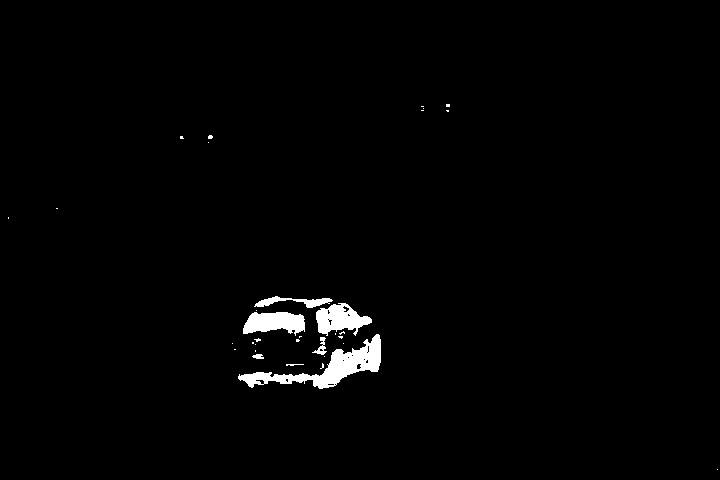
\includegraphics[width=5cm]{dataset/slike/bmd.jpg} }}
    \caption{Originalna slika i rezultat BMD algoritma}}
    \label{fig:example}
\end{figure}

\begin{figure}
    \centering
    \subfloat[GMM]{{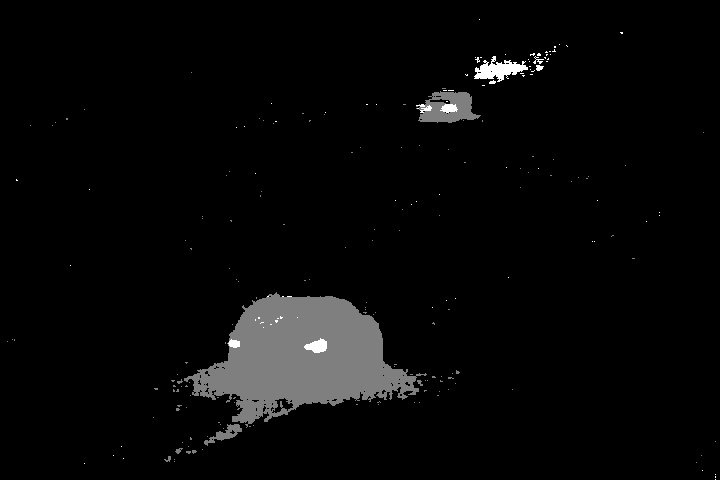
\includegraphics[width=5cm]{dataset/slike/mog2.jpg} }}
    \qquad
    \subfloat[KNN]{{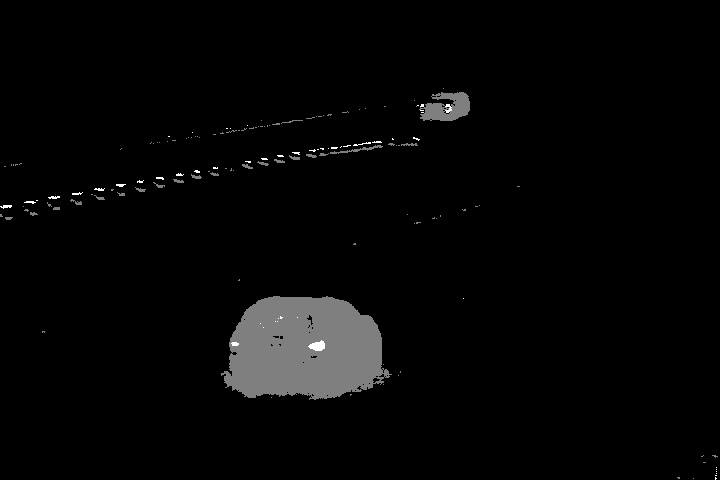
\includegraphics[width=5cm]{dataset/slike/knn.jpg} }}
    \caption{Rezultati GMM i KNN algoritama}}
    \label{fig:example}
\end{figure}

Algoritmi su pokretani na tri vrste test primera - saobraćaj za vreme mećave, saobraćaj u standardnim uslovima i noćni snimak nadzorne kamere. Svaki od algoritama je posmatran kao problem klasifikacije i za evaluaciju rezultata korišćene su mere \emph{Precision} i \emph{Recall}.

Ostvareni su sledeći rezulati:

\vspace{5mm}

\begin{tabular}{cc}
    \begin{minipage}{.5\linewidth}
        \begin{tabular}{|l|l|l|}
    \hline
\thead{BMD} & \thead{GMM} & \thead{KNN} \\ 
                    \hline
0.9409 & 0.4237 & 0.5218 \\    \hline
0.4757 & 0.1820 & 0.2738 \\    \hline
0.9822 & 0.8972 & 0.8872 \\    \hline
\end{tabular}
    \end{minipage} &

    \begin{minipage}{.5\linewidth}
        \begin{tabular}{|l|l|l|}
    \hline
\thead{BMD} & \thead{GMM} & \thead{KNN} \\ 
                    \hline
0.4528 & 0.9414 & 0.9157 \\    \hline
0.7833 & 0.8926 & 0.9025 \\    \hline
0.9436 & 0.7184 & 0.9068 \\    \hline
\end{tabular}
    \end{minipage} 
\end{tabular}




\end{document}
